\documentclass[border=2pt]{standalone}
\usepackage[T1]{fontenc}
\usepackage{times}
\usepackage{pgfplots}
\usepgfplotslibrary{groupplots}
\pgfplotsset{compat=1.18}
\definecolor{cA}{HTML}{2A78D6}
\definecolor{cB}{HTML}{EB6834}
\definecolor{cC}{HTML}{1BAF7A}
\definecolor{cD}{HTML}{EDA100}
\definecolor{cGrey}{HTML}{6F7988}
\definecolor{cLight}{HTML}{AEB4BD}
\definecolor{cRule}{HTML}{D9DEE5}
\pgfplotsset{every axis/.append style={font=\footnotesize, axis line style={cGrey}, tick style={cGrey},
  major grid style={cRule, line width=0.3pt}, ymajorgrids, tick pos=left, label style={font=\footnotesize},
  title style={font=\footnotesize\bfseries, yshift=-2pt}, legend style={font=\scriptsize, draw=none, fill=none}},
  err/.style={error bars/.cd, y dir=both, y explicit, error mark options={rotate=90, mark size=1.5pt}, /pgfplots/.cd}}
\begin{document}
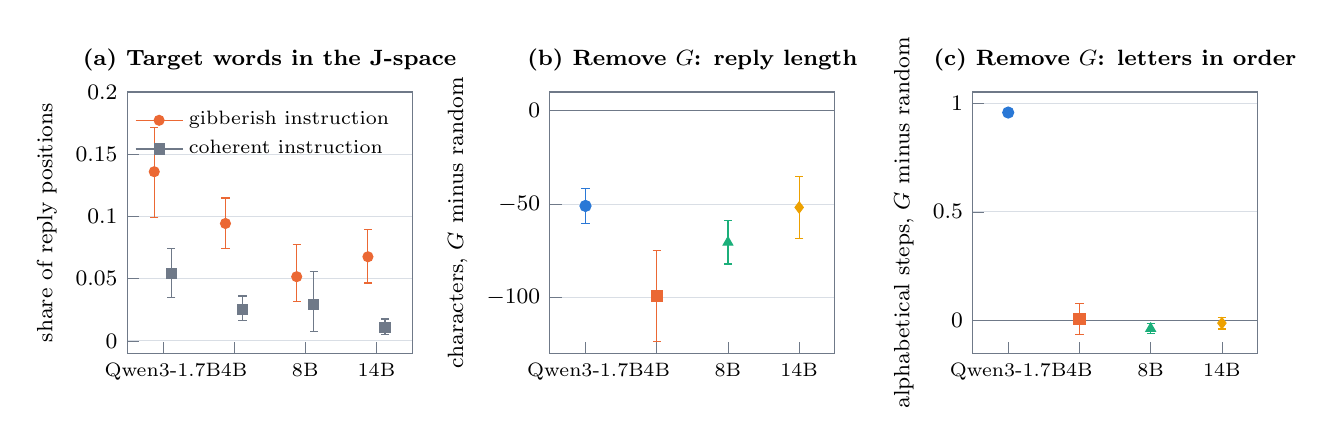
\begin{tikzpicture}
\begin{groupplot}[group style={group size=3 by 1, horizontal sep=1.75cm}, width=5.2cm, height=4.9cm, xtick={1,2,3,4}, xticklabels={Qwen3-1.7B,4B,8B,14B}, xmin=0.5, xmax=4.5, xticklabel style={font=\scriptsize},
  yticklabel style={/pgf/number format/fixed}]
\nextgroupplot[title={(a) Target words in the J-space}, ylabel={share of reply positions}, ymin=-0.01, ymax=0.2, legend pos=north east,
  legend cell align=left]
\addplot[color=cB, mark=*, mark size=1.8pt, err] coordinates {(0.8800,0.13596) += (0,0.03546) -= (0,0.03672)};\addlegendentry{gibberish instruction}
\addplot[color=cGrey, mark=square*, mark size=1.8pt, err] coordinates {(1.1200,0.05404) += (0,0.02001) -= (0,0.01883)};\addlegendentry{coherent instruction}
\addplot[color=cB, mark=*, mark size=1.8pt, err, forget plot] coordinates {(1.8800,0.09436) += (0,0.02048) -= (0,0.02042)};
\addplot[color=cGrey, mark=square*, mark size=1.8pt, err, forget plot] coordinates {(2.1200,0.02557) += (0,0.01052) -= (0,0.00938)};
\addplot[color=cB, mark=*, mark size=1.8pt, err, forget plot] coordinates {(2.8800,0.05160) += (0,0.02559) -= (0,0.02027)};
\addplot[color=cGrey, mark=square*, mark size=1.8pt, err, forget plot] coordinates {(3.1200,0.02894) += (0,0.02662) -= (0,0.02112)};
\addplot[color=cB, mark=*, mark size=1.8pt, err, forget plot] coordinates {(3.8800,0.06761) += (0,0.02191) -= (0,0.02106)};
\addplot[color=cGrey, mark=square*, mark size=1.8pt, err, forget plot] coordinates {(4.1200,0.01097) += (0,0.00660) -= (0,0.00609)};
\nextgroupplot[title={(b) Remove $G$: reply length}, ylabel={characters, $G$ minus random}, ymin=-130, ymax=10]
\draw[cGrey, line width=0.5pt] (axis cs:0.5,0) -- (axis cs:4.5,0);
\addplot[color=cA, mark=*, mark size=2pt, err] coordinates {(1.0000,-51.02283) += (0,9.57156) -= (0,9.57156)};
\addplot[color=cB, mark=square*, mark size=2pt, err] coordinates {(2.0000,-99.40065) += (0,24.44823) -= (0,24.44823)};
\addplot[color=cC, mark=triangle*, mark size=2pt, err] coordinates {(3.0000,-70.52197) += (0,11.63622) -= (0,11.63622)};
\addplot[color=cD, mark=diamond*, mark size=2pt, err] coordinates {(4.0000,-51.80817) += (0,16.52159) -= (0,16.52159)};
\nextgroupplot[title={(c) Remove $G$: letters in order}, ylabel={alphabetical steps, $G$ minus random}, ymin=-0.15, ymax=1.05]
\draw[cGrey, line width=0.5pt] (axis cs:0.5,0) -- (axis cs:4.5,0);
\addplot[color=cA, mark=*, mark size=2pt, err] coordinates {(1.0000,0.95590) += (0,0.01999) -= (0,0.01999)};
\addplot[color=cB, mark=square*, mark size=2pt, err] coordinates {(2.0000,0.00877) += (0,0.07132) -= (0,0.07132)};
\addplot[color=cC, mark=triangle*, mark size=2pt, err] coordinates {(3.0000,-0.03610) += (0,0.02473) -= (0,0.02473)};
\addplot[color=cD, mark=diamond*, mark size=2pt, err] coordinates {(4.0000,-0.01115) += (0,0.02706) -= (0,0.02706)};
\end{groupplot}
\end{tikzpicture}
\end{document}
